\section{Software Engineering Method}
This section will shortly describe the software engineering method used during this project. Many of these methods exist, such as Scrum, XP and the waterfall method, but we decided to use \ac{up} as the development method. In \ac{up} the software development process is divided into the following four phases: 

\begin{itemize}
\item[Inception] The project's boundaries and scope should be defined, as well as risk identification and preliminary project schedule.
\item[Elaboration] The team is expected to create the majority of the system requirements and establish the system architecture.
\item[Construction] This should be the largest phase in the project, since this is where the system is implemented.
\item[Transition] The project is deployed and feedback is incorporated into future releases.
\end{itemize}

Each phase is divided into iterations and will contain most of the activities associated with software development (analysis, design, implementation and testing), but to varying degrees. As can be seen in \autoref{fig:up}, the main focus will gradually shift from one activity to the next in the process.

\begin{figure}[hptb]
  \centering
    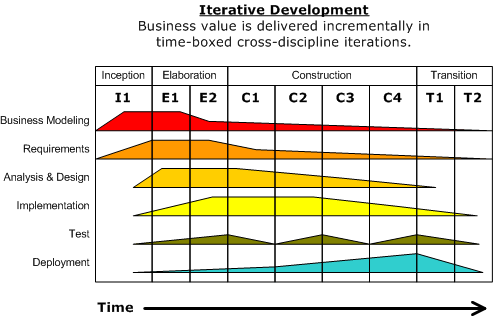
\includegraphics[width=\textwidth]{img/Development-iterative.png}
  \caption{Phases and activities in UP}
  \label{fig:up}
\end{figure}

Given that this project is estimated to require a long time spent on analysis before actual development can take place, an iterative method with short cycles spent on all activities, such as SCRUM, would not be a good idea. XP as a possible development method can also be discarded for the same reason. Instead the group will begin by focusing on the analysis, definition and scope of the problem to be solved. It will then move on to design of the solution along with prototype implementation and testing of these. Finally the product will be tested and findings during the testing will be implemented. 

The fact that \ac{up} is divided into phases that each have iterations fits well with the group's wish to focus mostly on one development activity at a time, without having a classical waterfall structure of the project.
